%& -shell-escape

% Les packages utilise's ci-dessous le sont a` titre indicatif ;
% vous pouvez les changer a` votre convenance.

% Le type de document: article, rapport...
\documentclass[a4paper]{report}

% Mettre les diffe'rents packages et fonctions que l'on utilise
%\usepackage[english]{babel}
%\usepackage[french]{babel}
%\usepackage{amsmath}
%\usepackage{amssymb}
%\usepackage{graphics,color}

% Commenter l'une de ces deux lignes
%\RequirePackage[applemac]{inputenc}
%\RequirePackage[latin1]{inputenc}

\usepackage[utf8]{inputenc}
\usepackage[english]{babel}
%\usepackage[francais]{babel}
\usepackage[T1]{fontenc}
%\usepackage{amsmath}
\usepackage{amsfonts}
\usepackage{amssymb}
\usepackage{placeins}
\usepackage{listings}
\usepackage{color}
\usepackage{textcomp}

%----- Package français
%\usepackage[utf8]{inputenc} %reconnaissance des accents
%\usepackage[francais]{babel} %document en français
%\usepackage[T1]{fontenc} %codage des fonts TeX ?



%----- math
\usepackage{amsmath}
\usepackage{dsfont}
\usepackage{calrsfs}

%----- images
\usepackage{graphicx}

%----- dot graphs
\usepackage{pgf}
\usepackage{tikz}
\usetikzlibrary{shapes,arrows}
%\usepackage[debug]{dot2texi}



%\title{Automatic test case generation for java}
%\author{Thomas BRIEN}
%\date{27 Mai 2013}

\begin{document}
%\maketitle

% Titre du rapport
\def\TitreRapport{
    Automatic test generation\\
    for OO programs
}

% Pre'nom et nom dde l'auteur
\def\NomsAuteurs{
    Thomas BRIEN
}

% Date du rapport (dans la me^me langue que le titre)
\def\DateRapport{
    27 Mai 2013
}

% Nom des encadrants
\def\Encadrants{
    \textbf{Tutor(s)} \\
    Arnaud MAKALA
}
% Nom du laboratoire
\def\Labo{
    Sopra Banking Software - R\&D
}

% mots clef
\def\keyWords{
    test generation, data generation, LTS, SMT solvers.
}


% Re'sume' en franc,ais avec mots-cle's
\def\ResumeFrancais{
La complexité des systèmes informatique devient de plus en plus importante, de même que les moyens qui doivent être mis en œuvre pour valider le bon fonctionnement des ces systèmes.
    Nous nous intéressons ici à l'automatisation des de la génération des cas de tests pour les programmes orientés objets. Le travaille effectué concerne les programmes java, les principes exposés s'applique à tout programme orienté objet.\\
    Il existe déjà des outils de génération de tests tel que \textit{Pex} et \textit{Sage}. Le travail qui suit est un état de l'art des techniques existantes et une proposition de théorie/prototype basé sur les algorithmes d'optimisation sous contrainte et les solveurs SMT.\\
    L'objectif est de proposer une méthode de génération des tests système, sans spécification. C'est à dire qu'on veut générer une suite de tests qui assure une non régression du système.
    \\[2mm]
    {\bf Mots-cl\'es : } \keyWords
}

\def\Abstract{
The complexity of software systems have considerably increased in the past decades and both the need and the difficulty of setting up correct test suits become more and more obvious.
    We are interested in the automation of test case generation for object oriented software. Our work is based on java code only, but principles are the same for every object oriented program.\\
    Some tools already handle the test case generation, such as \textit{Pex} or \textit{Sage}. In this paper, we establish a state of the art of test automation techniques and proposes a theory/prototype based on constraint optimisation algorithms and SMT solvers.\\
    The following work consists in setting up test suits at the system level, without specification. 
In other words, we want to generate a test suits that ensures the non-regression of he system, without any human intervention.
    \\[2mm]
    {\bf Key-words : } \keyWords
}


\thispagestyle{empty}
\begin{center}
\baselineskip=1.3\normalbaselineskip
{\bf\Large \TitreRapport}\\[8mm]
{\bf\large \NomsAuteurs}\\[1mm]
{\Labo}\\[4mm]
\DateRapport\\[4mm]
\Encadrants\\[10mm]

\newpage
{\bf R\'esum\'e}
\end{center}


\ResumeFrancais\\[4mm]
\newline
\begin{center}
{\bf Abstract}
\end{center}
\Abstract\\[4mm]

\newpage


\tableofcontents

\renewcommand{\thesection}{\arabic{section}}

\newtheorem{theorem}{Theorem}
\newtheorem{lemma}{Lemme}

\renewcommand{\thetheorem}{\empty{}}
\renewcommand{\thelemma}{\empty{}} 

\newenvironment{proof}[1][Proof]{\begin{trivlist}
\item[\hskip \labelsep {\bfseries #1}]}{\end{trivlist}}
\newenvironment{definition}[1][Definition]{\begin{trivlist}
\item[\hskip \labelsep {\bfseries #1}]}{\end{trivlist}}
\newenvironment{example}[1][Example]{\begin{trivlist}
\item[\hskip \labelsep {\bfseries #1}]}{\end{trivlist}}
\newenvironment{remark}[1][Rq:]{\begin{trivlist}
\item[\hskip \labelsep {\bfseries #1}]}{\end{trivlist}}
\newenvironment{rappel}[1][rappel:]{\begin{trivlist}
\item[\hskip \labelsep {\bfseries #1}]}{\end{trivlist}}


\chapter*{Introduction}
\addcontentsline{toc}{chapter}{Introduction}
The complexity of software systems have considerably increased in the past decades and both the need and the difficulty of setting up correct test suits become more and more obvious.
\newline
\textbf{Contribution :}\\
This paper proposes a model for white box testing of object oriented software.



%\chapter*{Plate-forme cible}
%\addcontentsline{toc}{chapter}{Plate-forme cible}




\chapter*{State of the art}
\addcontentsline{toc}{chapter}{State of the art}


\section*{Common tools and notions}
\addcontentsline{toc}{section}{Common tools and notions}

\subsection*{Unit tests with JUnit}
\addcontentsline{toc}{subsection}{Unit tests with JUnit}
Les tests unitaires ont pour but de prouver la validité d'un objet. Par exemple, on souhaite parcourir la totalité du code en lançant le programme avec des valeurs clef choisies par le programmeur chargé des tests.

\subsection*{Integration tests}
\addcontentsline{toc}{subsection}{Integration tests}
Les tests d'intégration visent à valider la bonne interaction entre plusieurs composants du système.

\subsection*{System tests}
\addcontentsline{toc}{subsection}{System tests}
Comme on peut s'en douter, les tests système permettent de contrôler le système dans son ensemble.

%\section*{Testing by contract}
%\addcontentsline{toc}{section}{Testing by contract}
%L'introduction de contrats dans le code permet de définir les conditions de début, de fin, et les constantes d'exécution.

\section*{Mutation testing}
\addcontentsline{toc}{section}{Mutation testing}
Mutation testing is a method that measures the "quality" of a test suite.\\
As detailed in $[2.1]$, the method consists in introducing small modification in the systeme (ex: switch a "+" into a "-") and run the test suite on the modified system, also called the mutant. If the test suite raises an failure, the mutant is "killed".\\
Of course, a test suite should test every possible action of the system and thus, should kill 100\% of mutants.

\section*{Test automation}
\addcontentsline{toc}{section}{Test automation}
- IOCO théorie\\
- ioLTS\\
- FSM/EFSM (Extended Finit State Machin)\\
- MBT (Model-Based Testing)\\
- SMT solvers (yices)\\

\subsection*{Software systems as LTSs}
\addcontentsline{toc}{subsection}{Software systems as LTSs}
A common theory for testing is based on \textit{labelled transition systems}.
\subsection*{Conformance testing}
\addcontentsline{toc}{subsection}{Conformance testing}





\chapter*{Idées et mise en œuvre}
\addcontentsline{toc}{chapter}{Idées et mise en œuvre}

\subsection*{Model of the system}
\addcontentsline{toc}{subsection}{Model of the system}

We are reasoning at the function level.\\
Every function can be represented as a labelled transition system. The set of labels is $L\ =\ I \cup U \cup A \cup D$ where :\\
\begin{itemize}
\item $I$ is a set of \textit{inputs} label
\item $U$ is a set of \textit{outputs} label
\item $A$ is a set of \textit{actions} label
\item $F$ is a set of \textit{formula} label
\end{itemize}
And the set of states is $S\ = C \cup D$\\
where $C$ is the set of common states and $D$ is the set of states preceding a \textit{decision}.
We call \textit{parent} of a label $f \in F$ a node $d \in D$ such as:\\
\[
\exists s \in S, 
d \xrightarrow{f} s\\
\]
$ $\\
\newline
The following graph represent a example function where:
\begin{itemize}
\item $I\ =\ \emptyset$
\item $U\ =\ \{out1, out2, out3, out4\}$
\item $A\ =\ \{act1, act2, act3\}$
\item $F\ =\ \{phi1, phi2, phi3\}$
\end{itemize}
$ $\\
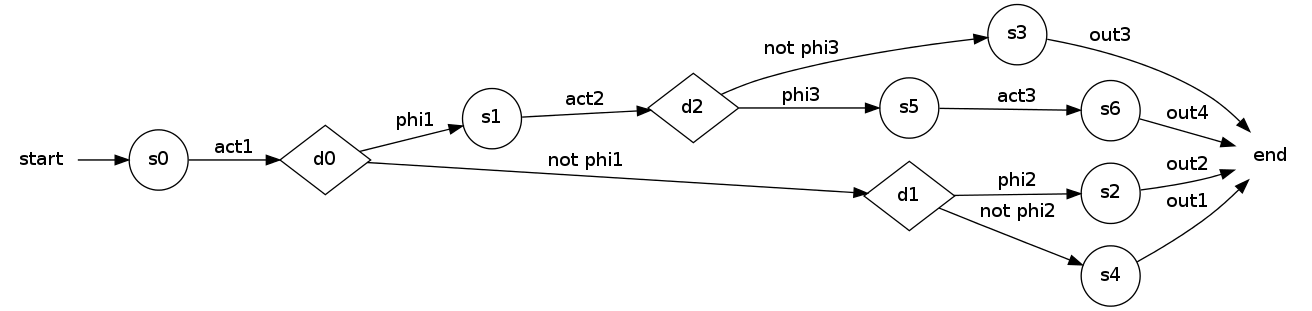
\includegraphics[scale=0.3]{../graphviz/LTSExample.png}
$ $\\
\newline

NB: The set of decisions label is associated with a set of state $\{d0, d1, d2\}$. Every transition from those states is a decision label i.e. \textbf{a first order formula}. We can also notice that decision states are the only multiple output states, and for a state $d$ with $n$ labels associated (every label corresponding to a FO formula $\phi_i$, $i\in[0, n]$)\\
\newline
1) For a set of inputs, the system is deterministic:\\
$\forall i, j \in [0, n], i \neq j \Rightarrow \neg (\phi_i \wedge \phi_j)$\\
\newline
2) every set of input lead to a computation:\\
$\forall i \in [0, n] $\\
\[\displaystyle \neg (\bigvee_{\substack{j=0 \\ j \neq i}}^{n} \phi_j) \Rightarrow \phi_i \]


\subsection*{Generation of initial test data}
\addcontentsline{toc}{subsection}{Generation of initial test data}




\subsection*{extracting sets suits with our model}
\addcontentsline{toc}{subsection}{extracting sets suits with our model}

\begin{itemize}
\item[$->$] random testing
\item[$->$] dynamic path construction leaded by coverage (récursive)
\item[$->$] logic modelisation (FOL) and SMT solver
\item[$->$] equivalent computation
\item[$->$] Bashir sliding
\end{itemize}


On raisonne sur le code source, et plus particulièrement sur des blocs de code. A partir de ce point, nous appellerons fonction élémentaire une partie de code dont la séquence d'exécution ne dépend d'aucune variable. Plus précisément, un code java qui ne contient pas d'accolades.\\
\newline
Par exemple, le code java suivant contient deux actions elementaires: val=arg1 et val+=arg2\\

\begin{lstlisting}
public int exemple(int arg1, int arg2){
		int val = 0;
		if(this.a<arg1){
			val = arg1;
		}
		if(val<arg2){
			val += arg2;
		}
		return val;
	}
\end{lstlisting}
A cette fonction, on associera le graph suivant:\\


\begin{figure}[h!]
   \caption{\label{étiquette} titre}
   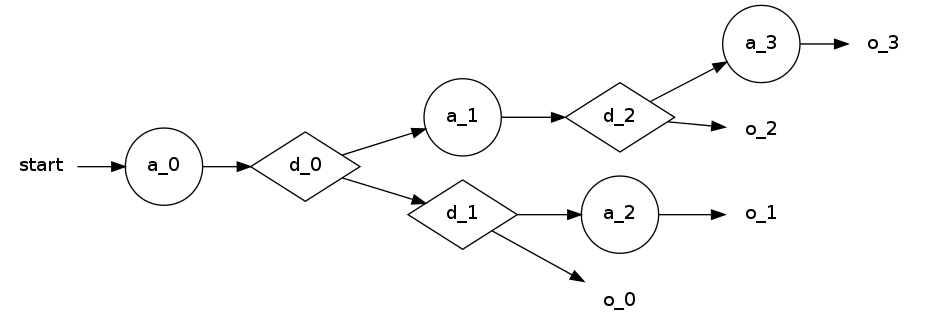
\includegraphics[scale=0.3]{../graphviz/doubleStackGraph.png}
\end{figure}
%\newline



En suivant notre modélisation, on obtient deux actions élémentaires:


\chapter*{Réalisations}
\addcontentsline{toc}{chapter}{Réalisations}



--- vous décrirez la problématique de recherche qui vous intéresse\\
\newline
L'automatisation à 100\% des tests pour les programmes orienté objets. Pour un tel niveau d'automatisation, on ne peut bien sûr pas espérer obtenir une spécification de l'utilisateur. Nous traitenons donc les tests de non régression pricipalement. Notre contribution est la suivante: nous ne nous limitons pas aux tests unitaires, mais on veut tester le bon fonctionnement d'un systeme entier. On veut donc mettre au point des tests d'intégration et systeme efficaces.\\
\newline
\newline
--- vous vous décrirez l'état de l'art\\
\newline
On se base sur la théorie \textbf{ioco}.\\
\newline
\newline
--- vous esquisserez les résultats que vous avez obtenus, ainsi que  les directions de recherche qu'il vous reste à explorer\\
\newline
\begin{itemize}
\item[$ 1) $] Pour un système simple, le problème est déjà résolu.
\item[$ 2) $] Pour un systeme complexe, on cherche à isoler des sous-systeme et à définir des relation de dépendence du type \textit{master/slave} entre ceux-ci.
\item[$ 3) $] On fait l'hypothèse que le code d'un sous-système est aussi la spécification attendu.
\item[$ 4) $] On lance des tests de conformance de la théorie \textbf{ioco} basé sur les spécification de chaques systèmes et leur relationde dépendence.
\end{itemize}
$ $\\
\newline
\newline
--- vous prendrez du temps pour expliquer les possibles écueils de ces directions de recherche et comment vous envisagez de les contourner.\\
\newline
Non non, pas d'écueils, j'te jure ;-)\\



\begin{figure}[h!]
   \caption{\label{étiquette} Exemple réel}
   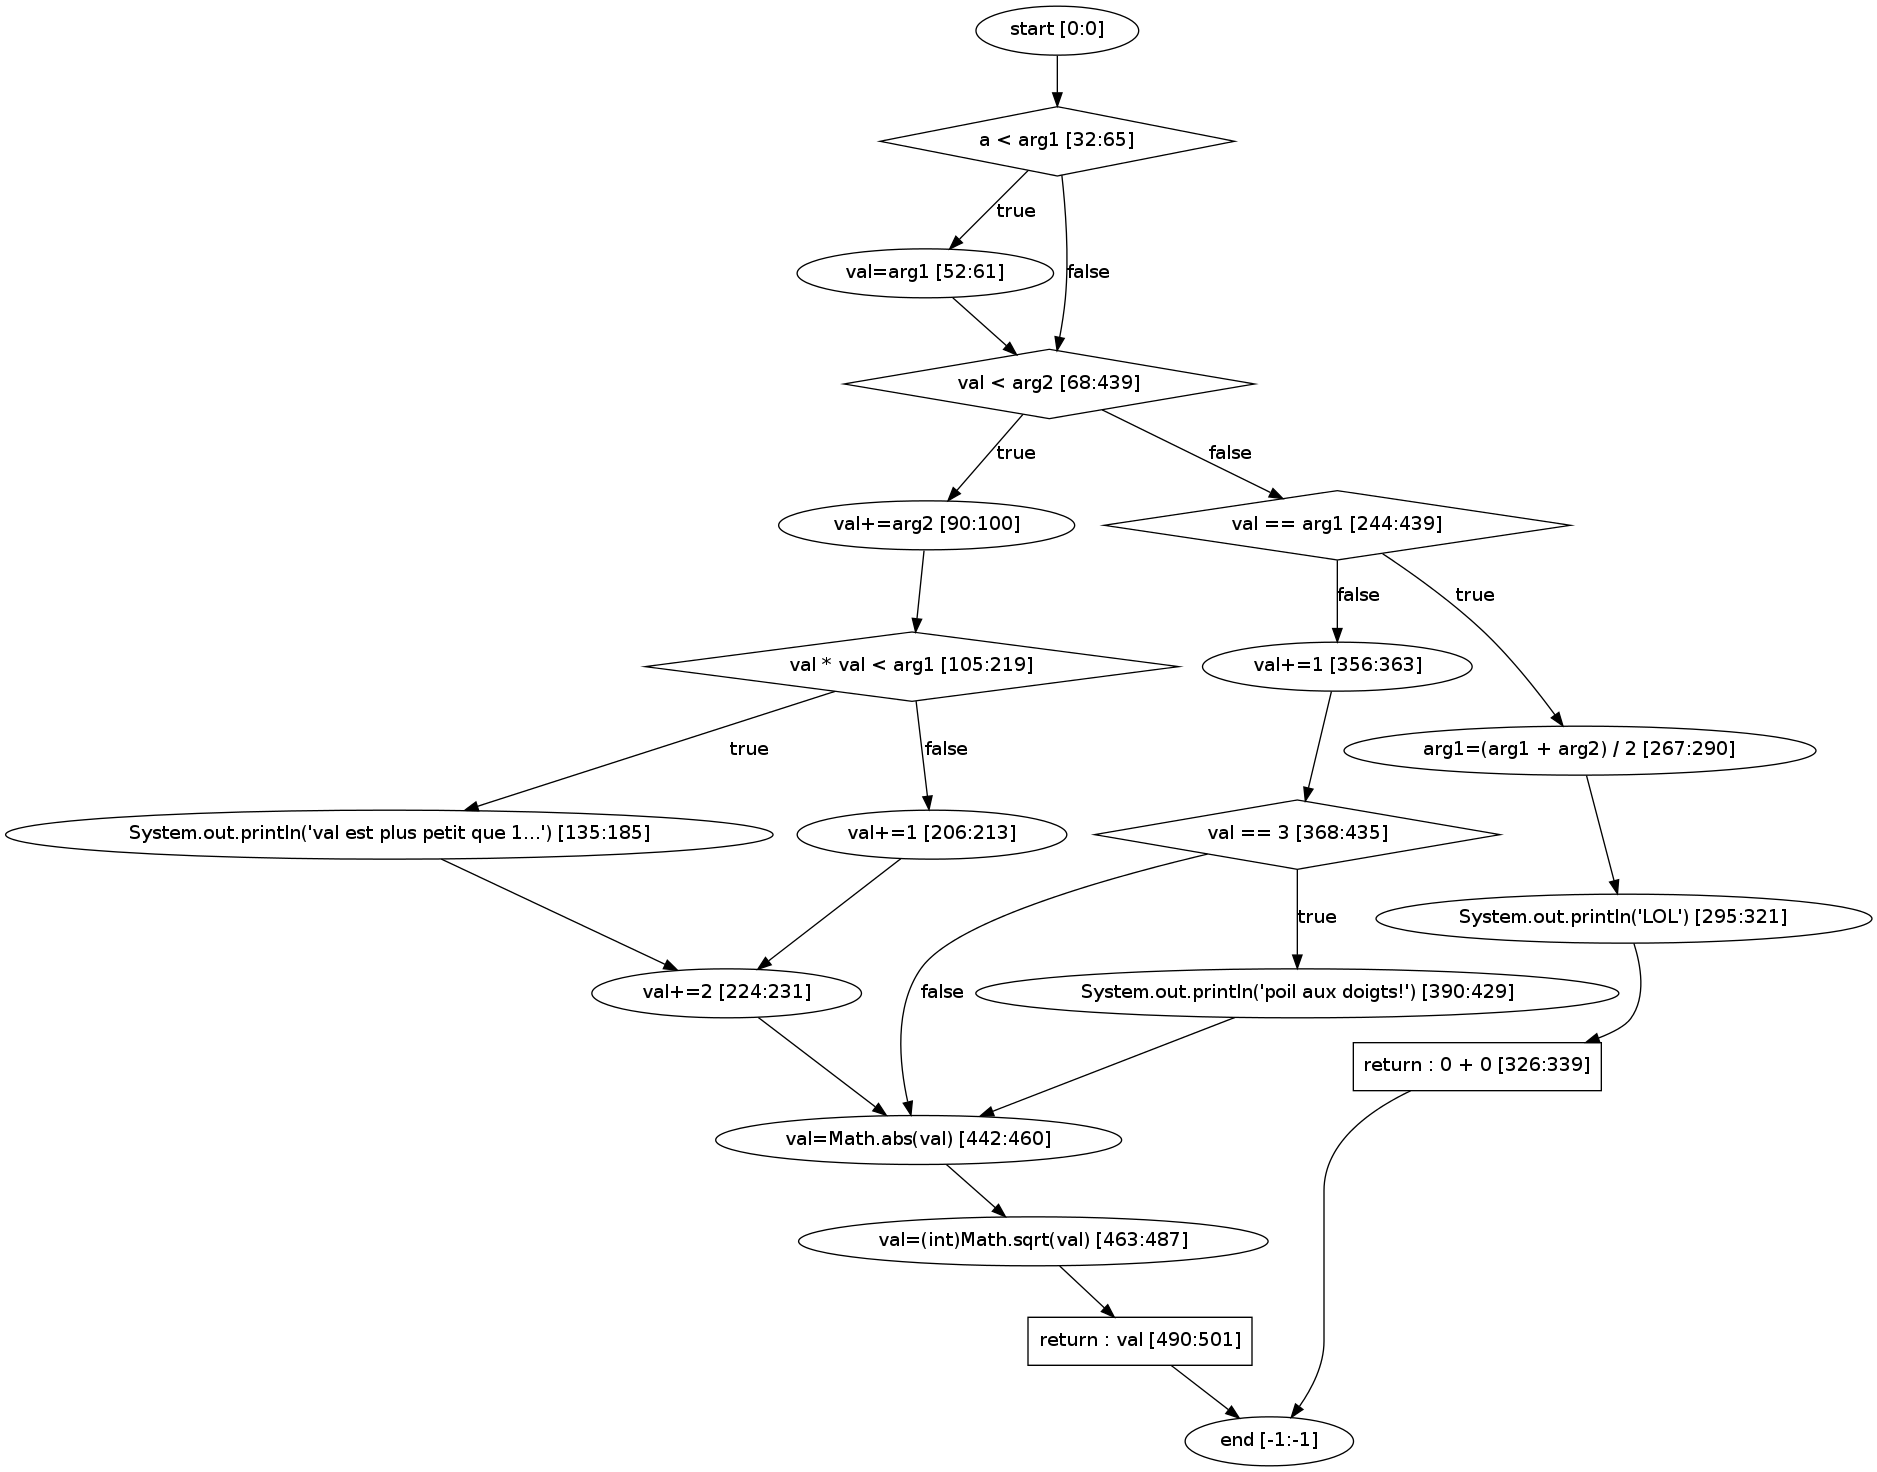
\includegraphics[scale=0.3]{../graphviz/realExemple.png}
\end{figure}

\chapter*{References}
\addcontentsline{toc}{chapter}{References}
\section*{BDD}
\addcontentsline{toc}{section}{BDD}
$[1.1]$ \textit{Testing by Contract
- Combining Unit Testing and Design by Contract}\\
Per Madsen (madsen@cs.auc.dk)
Institute of Computer Science, Aalborg University
Fredrik Bajers Vej 7, DK-9220 Aalborg, Denmark\\
\newline



\section*{Mutation testing}
\addcontentsline{toc}{section}{Mutation testing}
$[2.1]$ \textit{Composants objets fiables :
une approche pragmatique}\\
Daniel Deveaux* - Régis Fleurquin* - Patrice Frison*
Jean-Marc Jézéquel** - Yves Le Traon**\\
* Laboratoire VALORIA (Aglae)
UBS - IUP de Tohannic - Rue Mainguy
56000 VANNES\\
** IRISA-CNRS (Pampa)
Université Rennes 1 - Campus de Beaulieu
35042 RENNES\\
\newline

\section*{Automatisation}
\addcontentsline{toc}{section}{Automatisation}

$[3.1]$ Bertrand Meyer, Ilinca Ciupa, Andreas Leitner and Lisa (Ling) Liu, \textit{Automatic Testing of Object-Oriented Software}, in SOFSEM 2007\\
\newline
$[3.2]$ Hans-Gerhard Gross and Arjan Seesing, 
\textit{A Genetic Programming Approach to Automated Test Generation for Object Oriented Software}, Report TUD-SERG-2006-017\\
\newline
$[3.3]$\textit{Higher-Order Test Generation} - 
Patrice Godefroid - 
Microsoft Research\\
\newline


\end{document}